\section{Plotting Growth Curves}

After canopy analysis, the extracted canopy area measurements can be summarized
as growth curves as in \autoref{fig:growth-curve} The growth plotting script
reads canopy trait tables, groups measurements over time, estimates plant-level
growth rates, and produces a summary figure. The main figure shows canopy area
over time and the corresponding absolute growth rate. This allows users to
inspect both total plant size and the rate at which canopy area changes during
the experiment.

\begin{figure}[ht]
    \centering
    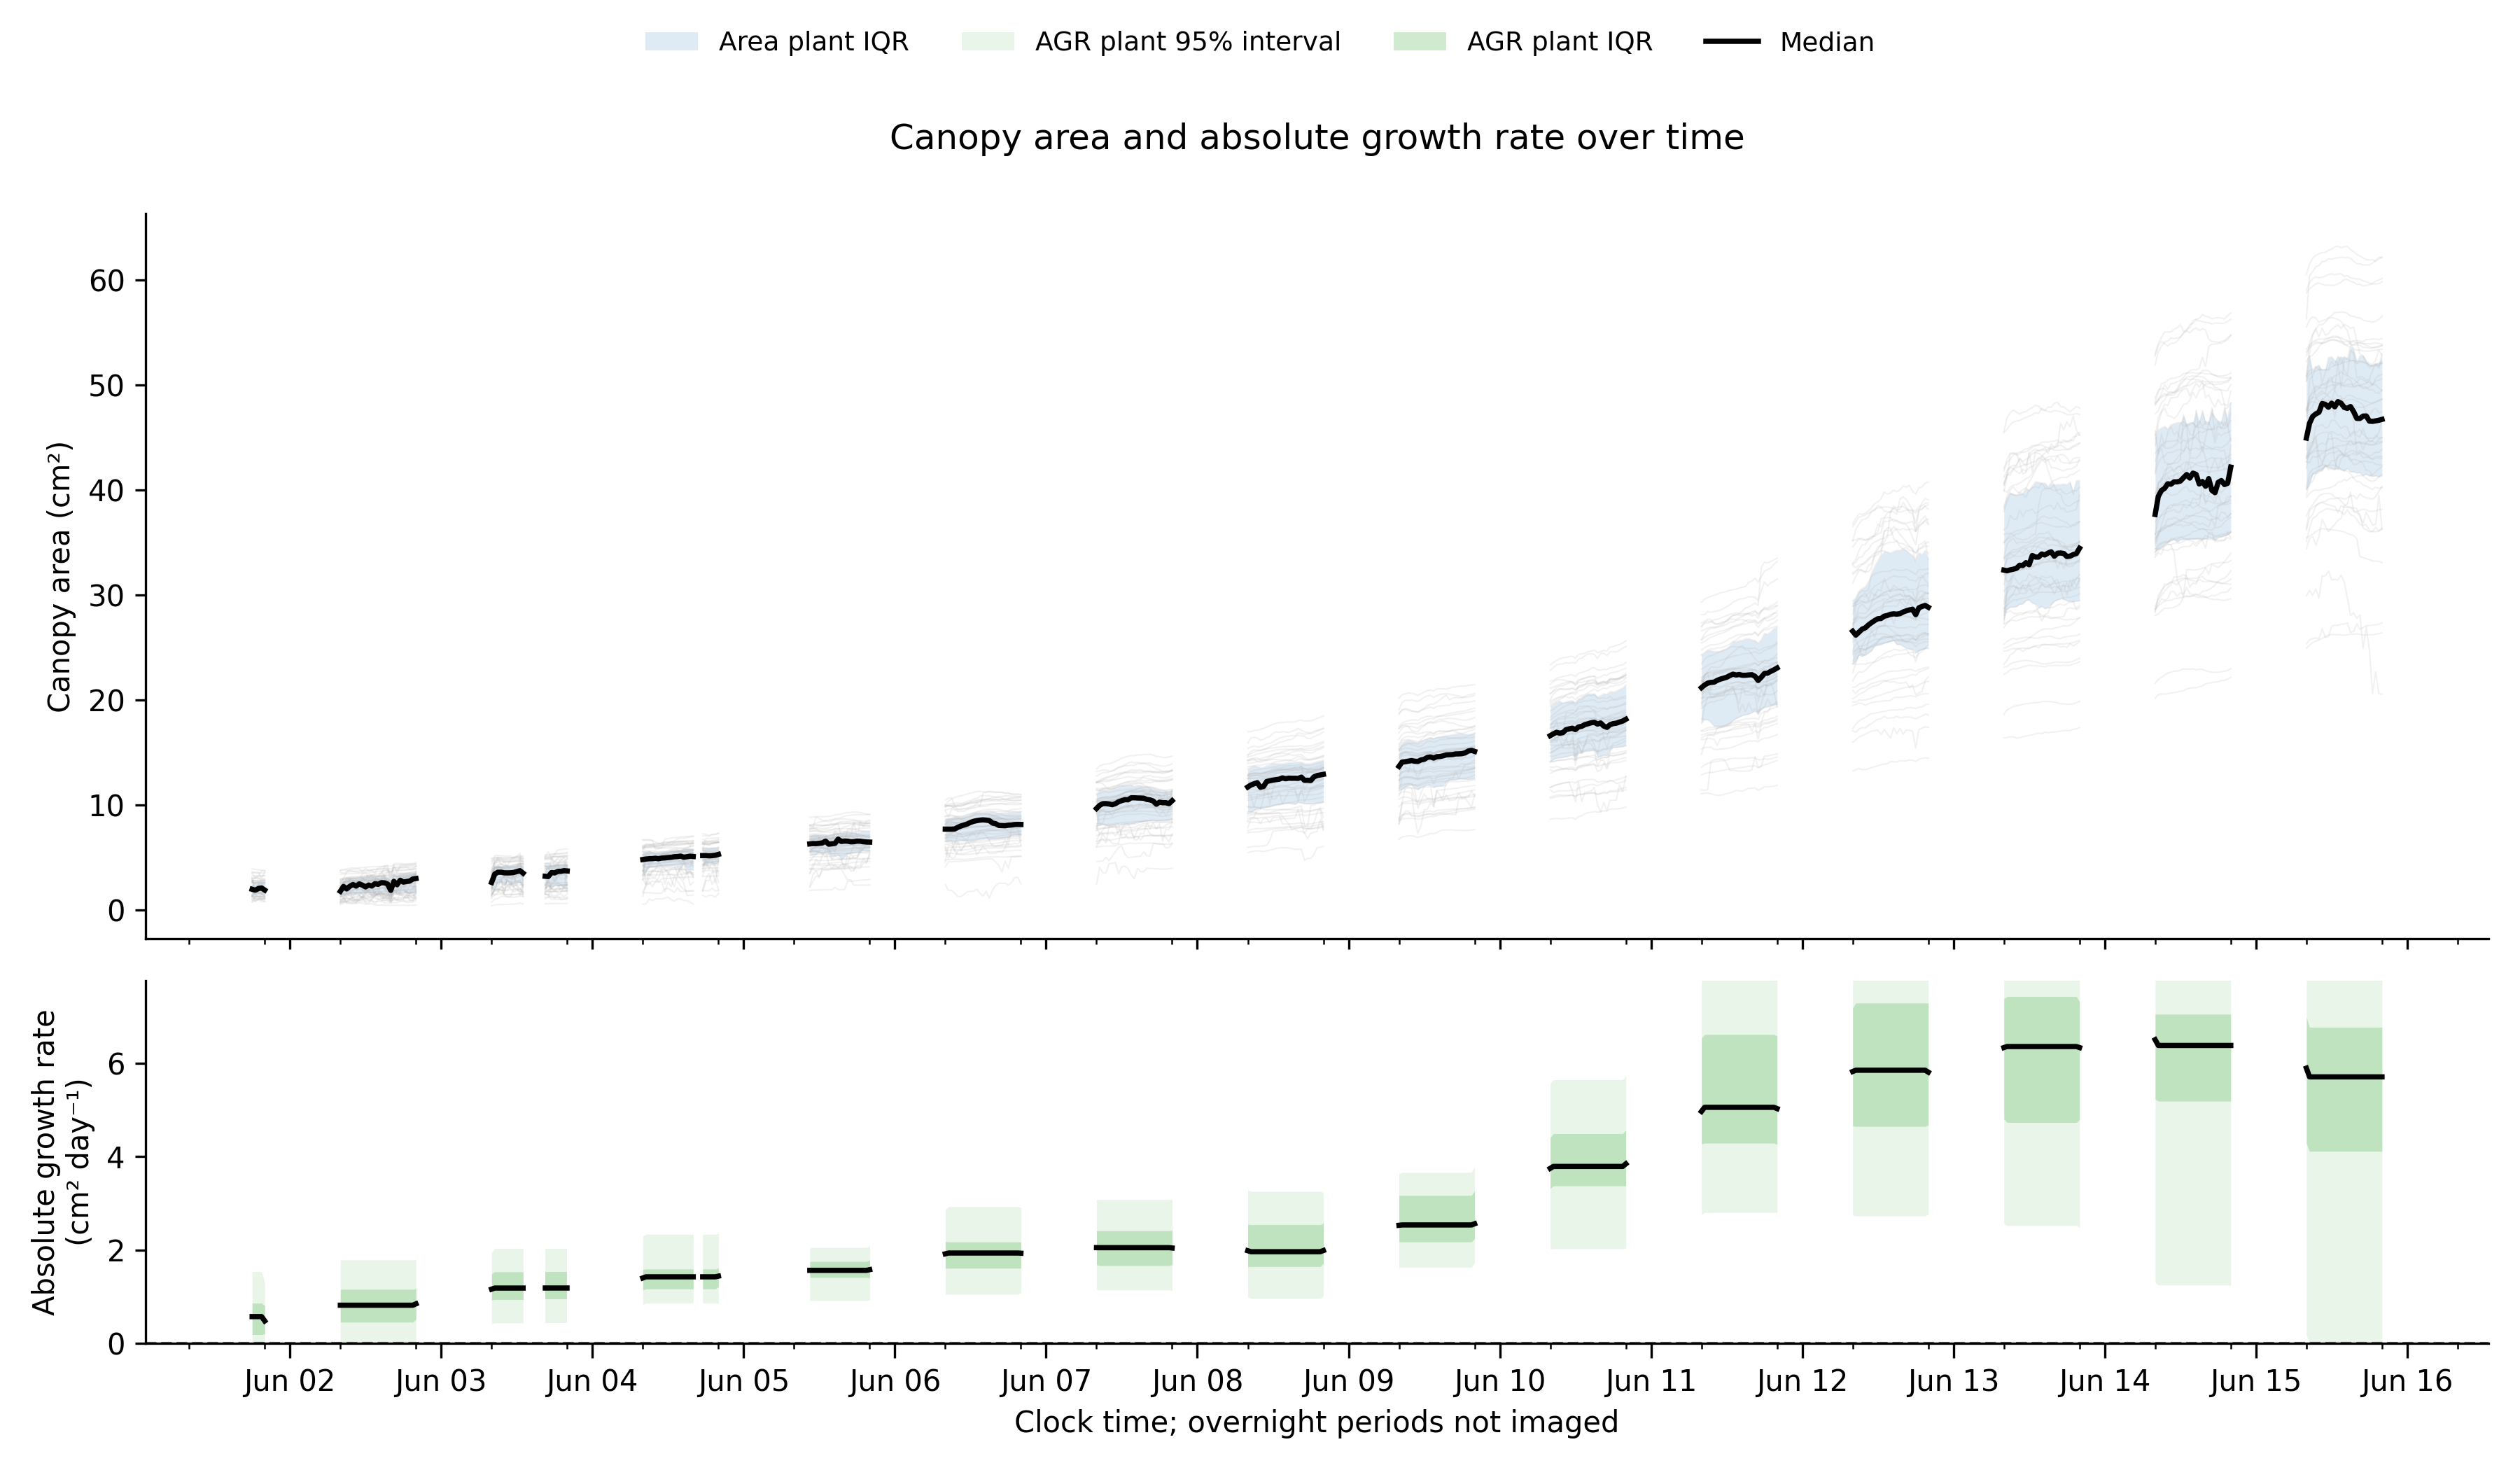
\includegraphics[width=\textwidth]{images/growth_curve.png}
    \caption{
        Example of a growth curve and rate speed plot generated from Phenopi
        data.
    }%
    \label{fig:growth-curve}
\end{figure}

\subsection{Input Data}

The growth plotting script can use either a combined trait table or a directory
containing individual trait files. The intended input is
\texttt{combined\_traits.csv} produced by the canopy analysis pipeline and
contains the extracted canopy traits for all processed images. The plotting
script uses the image timestamps and plant identifiers in this table to
reconstruct plant-level time series.

\subsection{Running the Growth Plot}

A typical command is shown below.

\begin{verbatim}
python -m scripts.plotting.plot_average_canopy_area \
  --input results/combined_traits.csv \
  --output results/canopy_area_absolute_growth.png \
  --summary-csv results/canopy_area_absolute_growth_summary.csv \
  --plant-curves-csv results/plant_absolute_growth_curves.csv \
  --growth-summary-csv results/absolute_growth_period_summary.csv \
  --growth-window-hours 24 \
  --growth-min-points 20
\end{verbatim}

The \texttt{--input} argument specifies the combined trait table. The
\texttt{--output} argument specifies the output figure. The remaining CSV
arguments define where summary tables should be written.

\subsection{Output Files}


The plotting script can produce several outputs:

\begin{verbatim}
canopy_area_absolute_growth.png
canopy_area_absolute_growth_summary.csv
plant_absolute_growth_curves.csv
absolute_growth_period_summary.csv
\end{verbatim}

The figure file shows the canopy area curve and absolute growth rate over time.
The summary CSV contains time-level summary statistics. The plant curves CSV
contains plant-level canopy area and growth-rate estimates. The growth summary
CSV contains period-level growth summaries that can be used for reporting or
further statistical analysis.

\subsection{Interpreting the Figure}

The upper panel shows canopy area over time. Individual plant curves are shown
as faint lines, while the central trend is shown as a stronger median line. The
shaded interval summarizes variation between plants. The lower panel shows the
absolute growth rate. Absolute growth rate describes how quickly canopy area
changes over time and is expressed in area per day. This can help identify
periods of slow growth, rapid growth, or growth reduction after treatment.
Because the experiment is only imaged during scheduled capture periods,
overnight periods are not directly observed. Apparent gaps in the time axis
therefore represent periods without image acquisition rather than missing
analysis output.

\subsection{Time Binning}

Technical replicate images can be collapsed into time bins before plotting. The
\texttt{--time-window} option controls the time window used to group nearby
measurements. For example, if several replicate images are taken around the
same scheduled time point, time binning prevents them from being treated as
independent time points in the plotted summary. Use a time window that is large
enough to group technical replicate captures, but small enough to avoid merging
biologically distinct imaging time points.

\subsection{Growth-Rate Settings}

Absolute growth rate is estimated from local windows along each plant curve.
The \texttt{--growth-window-hours} option defines the width of the centered
time window used for each local growth-rate estimate. A shorter window follows
rapid changes more closely but may produce noisier growth-rate estimates. A
longer window gives smoother estimates but may obscure short-term changes. The
\texttt{--growth-min-points} option defines the minimum number of measurements
required inside a local window. If too few points are available, the growth
rate is not estimated for that window. Increasing this value makes estimates
more conservative. Decreasing it allows more windows to be fitted, but may make
the estimates less stable.

\subsection{Treatment Periods}

Optional treatment start and end times can be supplied to mark a treatment
period in the output figure. For example, to add a treatment window between
2026-06-08 09:00 and 2026-06-10 20:00 to \autoref{fig:growth-curve}, we can use
the example below:

\begin{verbatim}
python -m scripts.plotting.plot_average_canopy_area \
  --input results/combined_traits.csv \
  --output results/canopy_area_absolute_growth.png \
  --summary-csv results/canopy_area_absolute_growth_summary.csv \
  --plant-curves-csv results/plant_absolute_growth_curves.csv \
  --growth-summary-csv results/absolute_growth_period_summary.csv \
  --growth-window-hours 24 \
  --growth-min-points 20
  --treatment-start "2026-06-08 09:00" \
  --treatment-end "2026-06-10 20:00"
\end{verbatim}

Which yields \autoref{fig:growth-curve-treatment}.

\begin{figure}[ht]
    \centering
    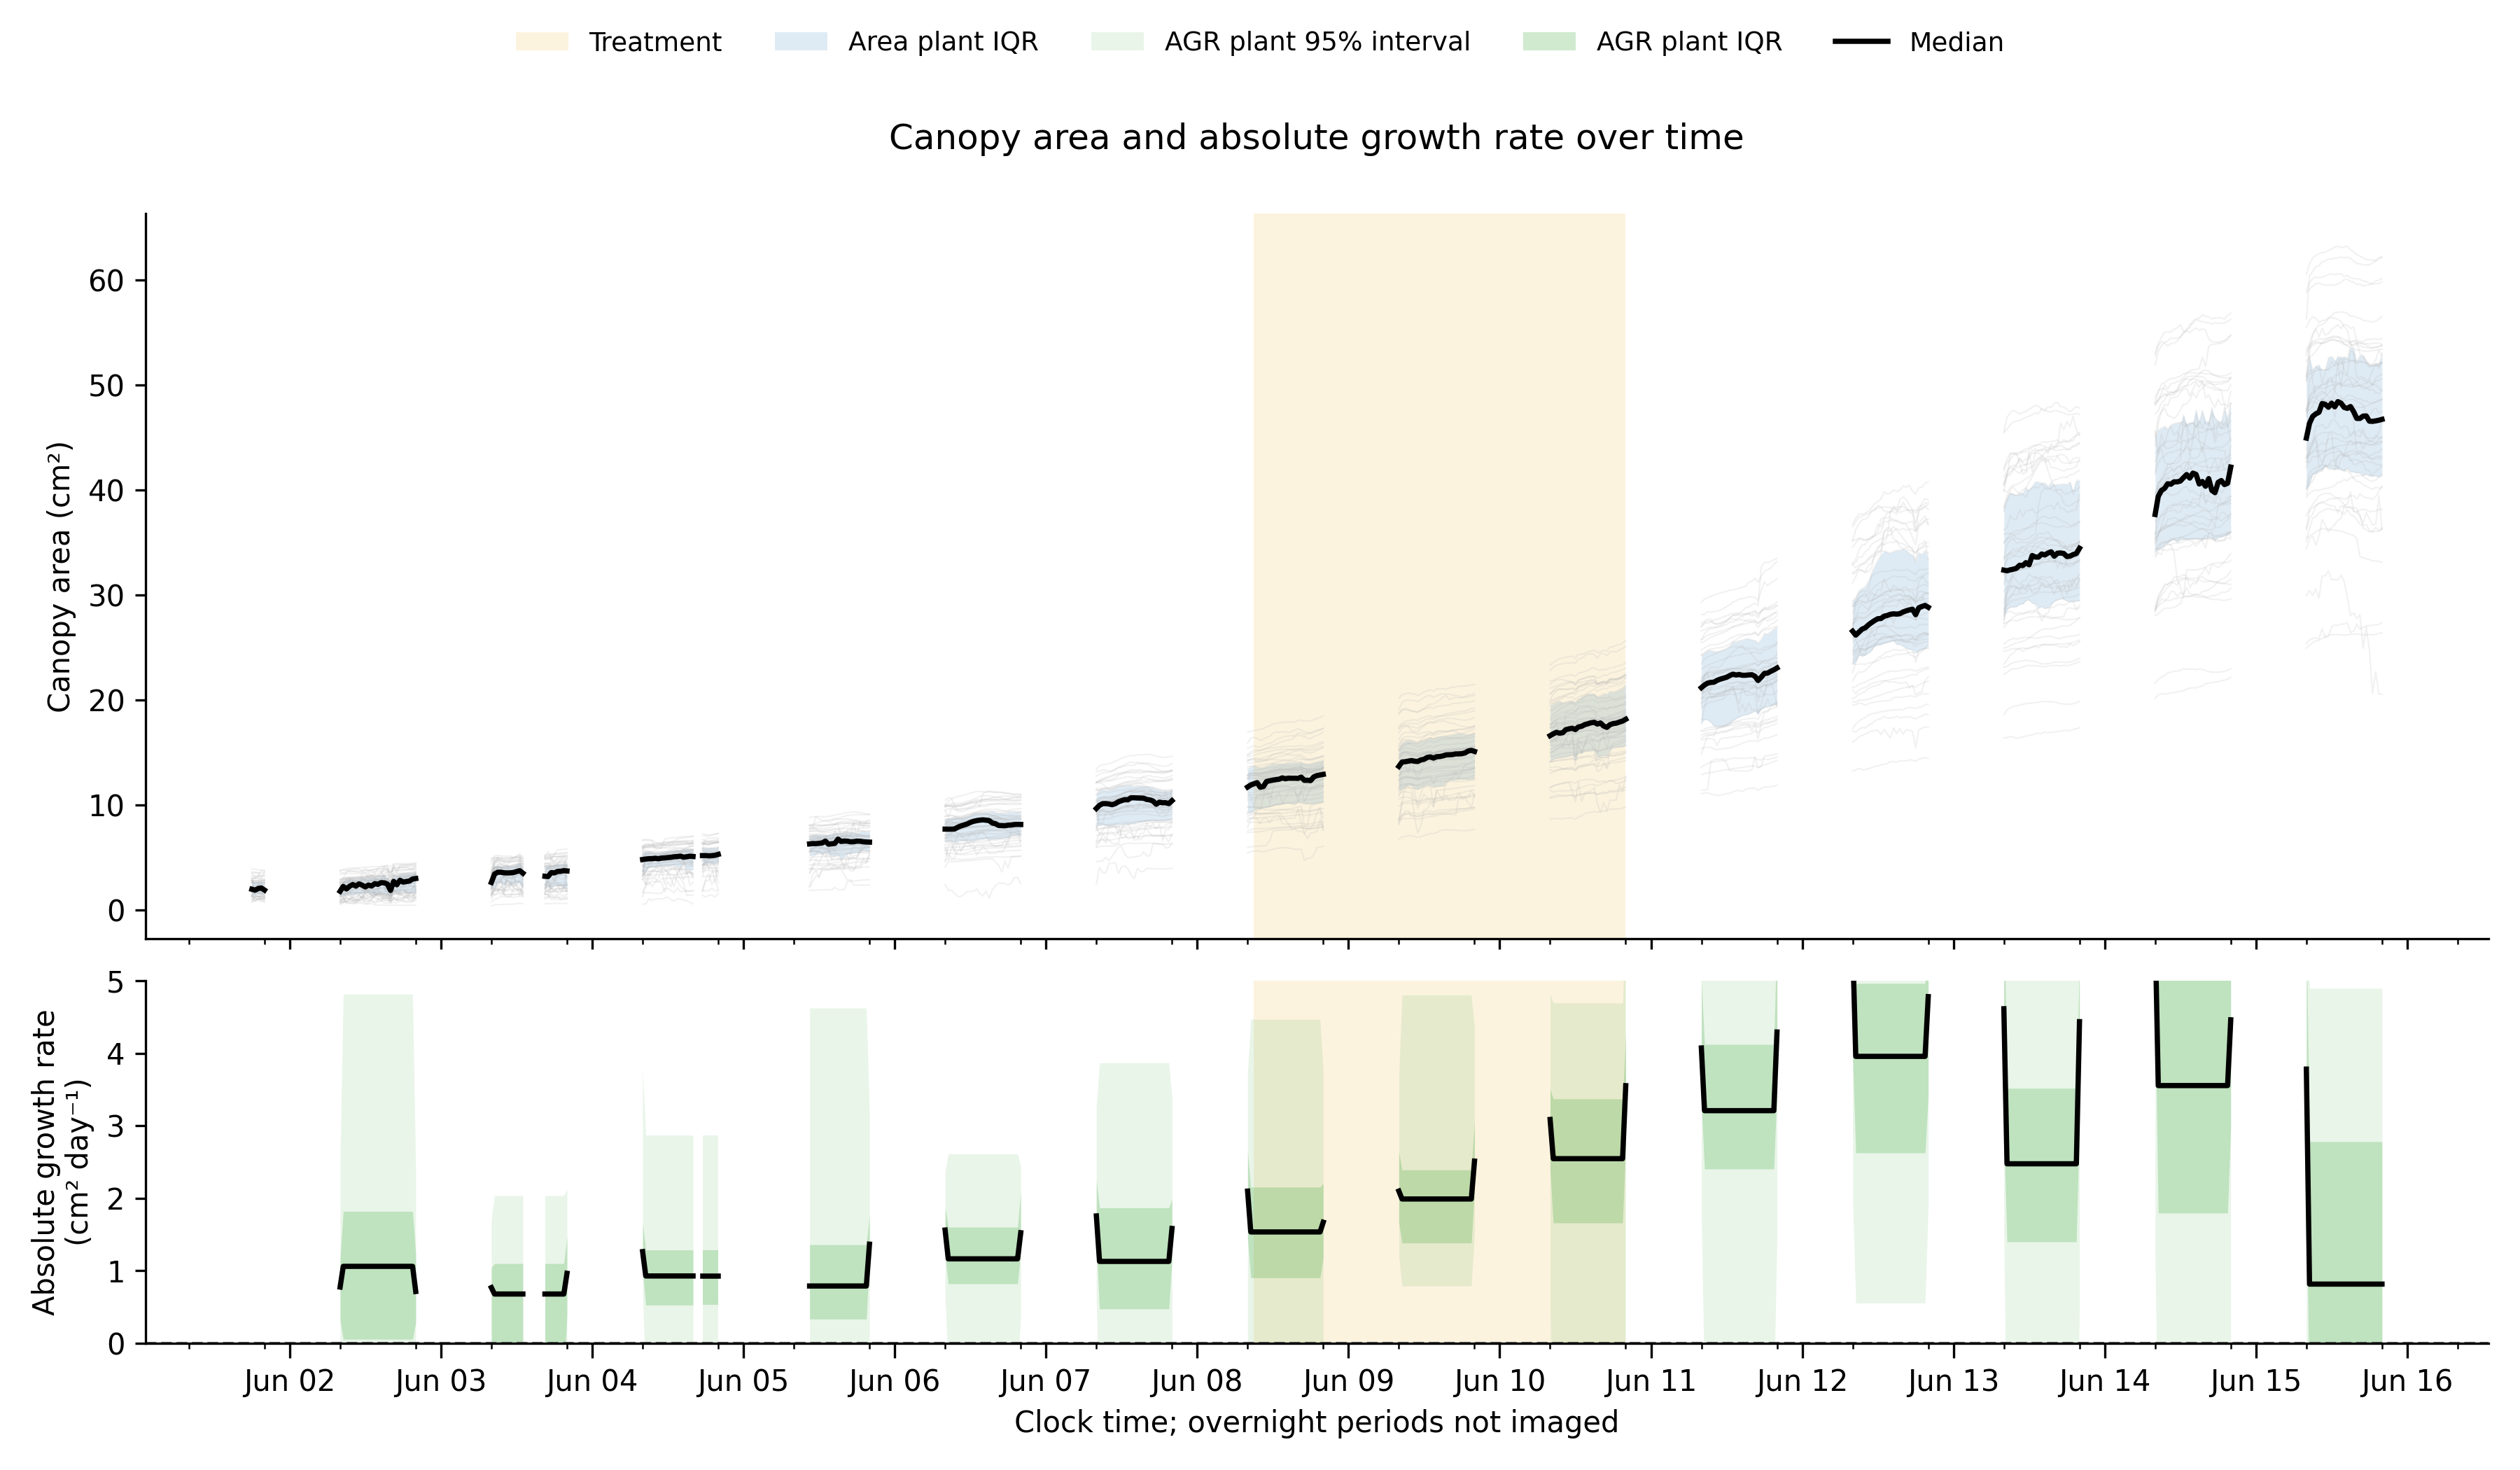
\includegraphics[width=\textwidth]{images/growth_curve_treatment.png}
    \caption{
        Example of a growth curve and rate speed plot generated from Phenopi
        data, with added treatment window.
    }%
    \label{fig:growth-curve-treatment}
\end{figure}

Treatment markers are useful when comparing growth before, during, and after an
experimental treatment. The supplied times should match the experiment timeline
and use the same date format as shown above. Currently, only a single treatment
window highlight is supported. 

\subsection{Interactive Display}

The plot can be shown interactively with \verb|--show|. This is useful during
exploratory analysis on a local computer. For automated or remote analysis, it
is usually better to write the figure directly to a file and inspect it
afterwards.

\subsection{Quality Checks}

Before interpreting growth curves, check that the plotted time range matches
the experiment, that the number of plant curves is reasonable, and that the
canopy area values are plausible. Sudden jumps or drops may indicate
segmentation errors, missing images, incorrect region assignment, or changes in
lighting. The growth-rate panel should be interpreted together with the canopy
area panel. A noisy growth-rate estimate is often caused by noisy canopy area
measurements. If the growth curve looks suspicious, return to the canopy
analysis overlays and inspect the corresponding images.
